%-----------------------------------LICENSE------------------------------------%
%   This file is part of Mathematics-and-Physics.                              %
%                                                                              %
%   Mathematics-and-Physics is free software: you can redistribute it and/or   %
%   modify it under the terms of the GNU General Public License as             %
%   published by the Free Software Foundation, either version 3 of the         %
%   License, or (at your option) any later version.                            %
%                                                                              %
%   Mathematics-and-Physics is distributed in the hope that it will be useful, %
%   but WITHOUT ANY WARRANTY; without even the implied warranty of             %
%   MERCHANTABILITY or FITNESS FOR A PARTICULAR PURPOSE.  See the              %
%   GNU General Public License for more details.                               %
%                                                                              %
%   You should have received a copy of the GNU General Public License along    %
%   with Mathematics-and-Physics.  If not, see <https://www.gnu.org/licenses/>.%
%----------------------------------Preamble------------------------------------%
\documentclass{book}
\usepackage{graphicx}   % Needed for figures.
\usepackage{amsmath}    % Needed for align.
\usepackage{amssymb}    % Needed for mathbb.
\usepackage{amsthm}     % For the theorem environment.
\usepackage[nottoc]{tocbibind} % Bibliography in toc.
\usepackage{hyperref}   % Hyperlinks for URLs and references.

% Setup parameters for hyperlinks.
\hypersetup{colorlinks = true, linkcolor = blue}

%------------------------Theorem Styles-------------------------%
\theoremstyle{plain}
\newtheorem{theorem}{Theorem}[section]

% Define theorem style for default spacing and normal font.
\newtheoremstyle{normal}
    {\topsep}               % Amount of space above the theorem.
    {\topsep}               % Amount of space below the theorem.
    {}                      % Font used for body of theorem.
    {}                      % Measure of space to indent.
    {\bfseries}             % Font of the header of the theorem.
    {}                      % Punctuation between head and body.
    {.5em}                  % Space after theorem head.
    {}

% Define default environments.
\theoremstyle{normal}
\newtheorem{examplex}{Example}[section]
\newtheorem{definitionx}{Definition}[section]
\newtheorem{notationx}{Notation}[section]

\newenvironment{example}{%
    \pushQED{\qed}\renewcommand{\qedsymbol}{$\blacksquare$}\examplex%
}{%
    \popQED\endexamplex%
}

\newenvironment{definition}{%
    \pushQED{\qed}\renewcommand{\qedsymbol}{$\blacksquare$}\definitionx%
}{%
    \popQED\enddefinitionx%
}

\newenvironment{notation}{%
    \pushQED{\qed}\renewcommand{\qedsymbol}{$\blacksquare$}\notationx%
}{%
    \popQED\endnotationx%
}

\title{Khovanov Homology and Legendrian Simple Knots}
\author{Ryan Maguire}
\date{\today}

% No indent and no paragraph skip.
\setlength{\parindent}{0em}
\setlength{\parskip}{0em}

\graphicspath{{images/}}

\begin{document}
    \pagenumbering{gobble}
    \begin{titlepage}
        \centering
        \LARGE{\bfseries{Khovanov Homology and Legendrian Simple Knots}}
        \par\vspace{3.5cm}
        \par\vspace{4cm}
        \Large{\itshape{Ryan Maguire}}
        \par\vspace{1.5ex}
        \normalsize{\today}
    \end{titlepage}
    \nopagecolor
    \pagenumbering{roman}
    \tableofcontents
    \listoffigures
    \listoftables
    \clearpage
    \chapter*{Preface}
        \addcontentsline{toc}{chapter}{Preface}
    \clearpage
    \chapter*{Acknowledgements}
        \addcontentsline{toc}{chapter}{Acknowledgements}
    \clearpage
    \pagenumbering{arabic}
    \chapter{Knots and Links}
        %-----------------------------------LICENSE------------------------------------%
%   This file is part of Mathematics-and-Physics.                              %
%                                                                              %
%   Mathematics-and-Physics is free software: you can redistribute it and/or   %
%   modify it under the terms of the GNU General Public License as             %
%   published by the Free Software Foundation, either version 3 of the         %
%   License, or (at your option) any later version.                            %
%                                                                              %
%   Mathematics-and-Physics is distributed in the hope that it will be useful, %
%   but WITHOUT ANY WARRANTY; without even the implied warranty of             %
%   MERCHANTABILITY or FITNESS FOR A PARTICULAR PURPOSE.  See the              %
%   GNU General Public License for more details.                               %
%                                                                              %
%   You should have received a copy of the GNU General Public License along    %
%   with Mathematics-and-Physics.  If not, see <https://www.gnu.org/licenses/>.%
%----------------------------------Preamble------------------------------------%
\begin{figure}
    \centering
    \begin{minipage}[b]{0.49\textwidth}
        \centering
        \resizebox{\textwidth}{!}{%
            \includegraphics{endless_knot_celtic_style.pdf}
        }
        \caption{Endless Knot}
        \label{fig:endless_knot_celtic_style}
    \end{minipage}
    \hfill
    \begin{minipage}[b]{0.49\textwidth}
        \centering
        \resizebox{\textwidth}{!}{%
            \includegraphics{basket_weave_knot_celtic_style.pdf}
        }
        \vspace{1.2em}
        \caption{Basket Weave Knot}
        \label{fig:basket_weave_knot_celtic_style}
    \end{minipage}
\end{figure}
\begin{figure}
    \centering
    \begin{minipage}[b]{0.49\textwidth}
        \centering
        \resizebox{\textwidth}{!}{%
            \includegraphics{borromean_rings_tricursal_valknut.pdf}
        }
        \caption{Tricursal Valknut}
        \label{fig:borromean_rings_tricursal_valknut}
    \end{minipage}
    \hfill
    \begin{minipage}[b]{0.49\textwidth}
        \centering
        \resizebox{\textwidth}{!}{%
            \includegraphics{borromean_rings_no_shadow.png}
        }
        \caption{Tubular Borromean Rings}
        \label{fig:borromean_rings_no_shadow}
    \end{minipage}
\end{figure}
\begin{figure}
    \centering
    \begin{minipage}[b]{0.49\textwidth}
        \centering
        \resizebox{\textwidth}{!}{%
            \includegraphics{trefoil_knot_celtic_style.pdf}
        }
        \caption{Celtic Trefoil}
        \label{fig:trefoil_knot_celtic_style}
    \end{minipage}
    \begin{minipage}[b]{0.49\textwidth}
        \centering
        \resizebox{\textwidth}{!}{%
            \includegraphics{trefoil_unicursal_valknut.pdf}
        }
        \caption{Unicursal Valknut}
        \label{fig:trefoil_unicursal_valknut}
    \end{minipage}
\end{figure}
Knots have long been marveled as a source of art and beauty. The Book of
Kells, a Celtic rendition of the four gospels of the New Testament created
between the $7^{\small\textrm{th}}$ and $9^{\small\textrm{th}}$
centuries \cite[p.~108]{Nordenfalk1977}, contains intricate drawings of
complicated knots and links. Many pages depict the endless knot
(Fig.~\ref{fig:endless_knot_celtic_style}) and the basket weave knot
(Fig.~\ref{fig:basket_weave_knot_celtic_style}). The endless knot also appears
in Tibetan Buddhism, being one of the ``eight auspicious symbols''
\cite[p.~11]{BeerTibetanSymbols}. The Borromean rings
(Fig.~\ref{fig:borromean_rings_no_shadow}) are found in Celtic, Tibetan,
and Viking cultures
\cite[p.~129]{VikingWomenJesch}%
\footnote{%
    The Legend of Hildr is depicted on the stone carving in this
    reference. The tricursal \textit{Valknut}
    (Fig.~\ref{fig:borromean_rings_tricursal_valknut}),
    the Viking-Germanic version of Borromean rings,
    can be seen on the third carving from the top.
},
and the trefoil in Celtic (Fig.~\ref{fig:trefoil_knot_celtic_style}),
Islamic, Norse (Fig.~\ref{fig:trefoil_unicursal_valknut}), and Tibetan art.
\par\hfill\par
As a mathematical discipline, the origins of knot theory
date back to the $18^{\small\textrm{th}}$ and
$19^{\small\textrm{th}}$ centuries with semi-rigorous treaties of
the subject being formed by Vandermonde (1735-1796 C.E.) in 1771
\cite{Vanermonde1771} and Gauss
(1777-1855 C.E.) in 1833 \cite[p.~1327]{RiccaNipotaGaussLinkingNumber}.
James Clerk Maxwell (1831-1879 C.E.) reinterpreted Gauss' work for the theory
of electromagnetism in his seminal 1873 work
\textit{A Treatise on Electricity and Magnetism}
\cite{MaxwellTreatist1873}.
Serious investigations into the field are often first attributed to Peter Tait
(1831-1901 C.E.) who established some of the earliest tabulations of knots
in 1885 \cite{TaitOnKnots1885}. He also put forward several conjectures,
the \textit{Tait conjecture}, that were proved in the 1980s and 1990s by
REFERENCE 1, REFERENCE 2, and REFERENCE 3.
\par\hfill\par
Tait was motivated by Lord Kelvin's hypothesis that chemical properties
of matter could be explained by atoms being \textit{knotted}
\cite{ThompsonVortex1867}, in some sense. J.J. Thompson expanded this idea and
developed some of the earlier mathematical properties of knots
\cite{ThompsonVortexRings1883}, only to abandon the hypothesis altogether with
his discovery of the electron \cite{ThompsonStructureOfAtoms1904}.\footnote{%
    This article also contains the famous \textit{Thompson problem}, asking for
    the minimum equilibrium configuration for $n$ equally charged particles
    constrained to a lie on a sphere.
}
And so vortex theory died, but knot theory lived on as it became a part of
\textit{topology}, which was being brought to the main stage of mathematics
by Henri Poincar\'{e}'s famous \textit{analysis situs}
\cite{PoincareAnalysisSitus1895}. Within the following decades mathematicians
such as James Alexander (1888-1971 C.E.), R. H. Bing (1914-1986 C.E.),
Max Dehn (1878-1952 C.E.), Heinz Hopf (1894-1971 C.E.),
Kurt Reidemeister (1893-1971 C.E.), Herbert Seifert (1907-1996 C.E.),
and James Whitehead (1904-1960 C.E.) began making serious and rigorous strides
into the theory.

        %-----------------------------------LICENSE------------------------------------%
%   This file is part of Mathematics-and-Physics.                              %
%                                                                              %
%   Mathematics-and-Physics is free software: you can redistribute it and/or   %
%   modify it under the terms of the GNU General Public License as             %
%   published by the Free Software Foundation, either version 3 of the         %
%   License, or (at your option) any later version.                            %
%                                                                              %
%   Mathematics-and-Physics is distributed in the hope that it will be useful, %
%   but WITHOUT ANY WARRANTY; without even the implied warranty of             %
%   MERCHANTABILITY or FITNESS FOR A PARTICULAR PURPOSE.  See the              %
%   GNU General Public License for more details.                               %
%                                                                              %
%   You should have received a copy of the GNU General Public License along    %
%   with Mathematics-and-Physics.  If not, see <https://www.gnu.org/licenses/>.%
%----------------------------------Preamble------------------------------------%
\section{Basic Definitions}
    Following \cite[p.~15]{LivingstonKnotTheory}, we define a knot as follows.
    \begin{definition}[\textbf{Knot}]
        A knot is a polygonal (piece-wise linear) embedding
        $\gamma:\mathbb{S}^{1}\rightarrow\mathbb{R}^{3}$ of the unit circle
        into three dimensional Euclidean space.
    \end{definition}
    A triangle serves as a polygonal example of the unknot, and the trefoil is
    given a polygonal embedding in Fig.~\ref{fig:trefoil_knot_polygonal}.
    \begin{figure}
        \centering
        \resizebox{0.4\textwidth}{!}{%
            \includegraphics{trefoil_knot_polygonal.pdf}
        }
        \caption{Polygonal Trefoil Knot}
        \label{fig:trefoil_knot_polygonal}
    \end{figure}
    While it is possible to define knots using \textit{continuous} embeddings,
    such a definition provides for the existence of
    \textit{wild knots} \cite{FoxArtinWildKnots1948}.\footnote{%
        See \cite{BrowneWildKnots} for how to procedurally generate wild knots.
    }
    \textit{Smooth} embeddings can similarly be used, albeit at the expense of
    a slightly harder definition of \textit{knot equivalence}. In the polygonal
    case this comes with ease. Given a piece-wise linear embedding
    $\gamma:\mathbb{S}^{1}\rightarrow\mathbb{R}^{3}$ with vertices
    $P_{0},\,\dots,\,P_{n-1}$ we are allowed to deform $\gamma$ into a new
    embedding $\gamma'$ formed by the (ordered) vertices
    $P_{0},\,\dots,\,P_{n-1},\,P_{n}$
    such that the triangle $\Delta{P}_{n-1}P_{n}P_{0}$ (interior included)
    only intersects $\gamma$
    along the line segment $P_{0}P_{n-1}$. This is called an
    \textbf{elementary knot equivalence}. With this we define equivalent knots.
    \newpage
    \begin{definition}[\textbf{Equivalent Knots}]
        Equivalent knots are polygonal embeddings
        $\gamma,\gamma':\mathbb{S}^{1}\rightarrow\mathbb{R}^{3}$ that differ by
        a finite number of elementary knot equivalences.
    \end{definition}
    A triangle and a square are equivalent knots, as are all regular
    polygons in the plane, which serve as examples of the unknot.
    Moreover, by the Jordan curve theorem any two embeddings that
    lie in a plane $S\subseteq\mathbb{R}^{3}$ are equivalent to the unknot as
    well. Application of Chazelle's algorithm
    \cite{ChazelleTriangulationAlgorithm} tells us this equivalence
    can be demonstrated in linear time.\footnote{%
        Explicitly, use Chazelle's algorithm to triangulate the polygonal
        figure. \textit{Collapse} any triangle with a vertex on the boundary
        of the polygon making an acute angle by deleting said vertex.
        Continue doing this until there is one triangle left.
        Both Chazelle's algorithm and this collapsing
        process run in linear time. Equivalence of two triangles in the
        plane can be done in constant time.
    }
    \par\hfill\par
    Knot equivalence induces an equivalence relation on the set of all knots,
    and this motivates a definition.
    \begin{definition}[\textbf{Knot Type}]
        The knot type of a knot $\gamma:\mathbb{S}^{1}\rightarrow\mathbb{R}^{3}$
        is the equivalence class $\mathcal{K}=[\gamma]$ of all knots that are
        equivalent to $\gamma$.
    \end{definition}
    Many texts do not distinguish between a knot and its knot type.
    While the polygonal definitions of knot and knot equivalence are perhaps
    the easiest to describe, it is also convenient to think of knots as smooth
    embeddings of $\mathbb{S}^{1}$ into $\mathbb{R}^{3}$. Indeed, most of the
    figures to follow will depict smooth knots. It is then fortunate that the
    two descriptions are equivalent for most purposes, and both exclude the
    existence of wild knots \cite[p.~147]{CrowellFoxKnotTheory}. As mentioned,
    the smooth setting has a more verbose definition of knot equivalence.
    Smooth embeddings $\gamma,\gamma':\mathbb{S}^{1}\rightarrow\mathbb{R}^{3}$
    are considered equivalent if there is an \textit{ambient isotopy}
    between them. The definition is quite precise.
    \newpage
    \begin{definition}[\textbf{Ambient Isotopy}]
        An ambient isotopy from a smooth embedding
        $\gamma:\mathbb{S}^{1}\rightarrow\mathbb{R}^{3}$ to a smooth
        embedding $\gamma':\mathbb{S}^{1}\rightarrow\mathbb{R}^{3}$ is a
        smooth function
        $H:\mathbb{R}^{3}\times[0,\,1]\rightarrow\mathbb{R}^{3}$
        such that for each $t\in[0,\,1]$ the function
        $H_{t}:\mathbb{R}^{3}\rightarrow\mathbb{R}^{3}$ defined by
        $H_{t}(\mathbf{x})=H(\mathbf{x},\,t)$ is a diffeomorphism,
        and such that:
        \begin{subequations}
            \begin{align}
                H_{0}\big((x,\,y,\,0)\big)&=\gamma\big((x,\,y)\big)\\
                H_{1}\big((x,\,y,\,0)\big)&=\gamma'\big((x,\,y)\big)
            \end{align}
        \end{subequations}
        for each $(x,\,y)\in\mathbb{S}^{1}$. Smoothness of $H$ is taken in
        the sense of the product smooth structure between a smooth manifold and
        a smooth manifold with boundary.
    \end{definition}
    An ambient isomorphism is a smooth family of diffeomorphisms that
    drags the first (smooth) knot to the second. A comment on this.
    Alternative and inequivalent definitions do exist in the literature.
    The definition in \cite[p.~4]{CrowellFoxKnotTheory}, for example,
    requires a single diffeomorphism
    $f:\mathbb{R}^{3}\rightarrow\mathbb{R}^{3}$ that
    takes the image of $\gamma$ to the image of $\gamma'$. Such a
    definition is unable to distinguish a knot from its \textit{mirror},
    the result of composing the knot with the reflection $z\mapsto{-z}$.
    If one requires $f$ be \textit{orientation preserving}, then the
    two definitions are equivalent.
    \begin{definition}[\textbf{Smoothly Equivalent Knots}]
        Smoothly equivalent knots are smooth embeddings
        $\gamma:\mathbb{S}^{1}\rightarrow\mathbb{R}^{3}$ and
        $\gamma':\mathbb{S}^{1}\rightarrow\mathbb{R}^{3}$ such that there
        exists an ambient isotopy between them.
    \end{definition}
    As in the polygonal case, smooth equivalence yields an equivalence
    relation. Any smooth knot can be made polygonal by choosing a sufficiently
    small enough $\varepsilon>0$ and sampling the embedding such that no two
    successive points are more than $\varepsilon$ apart, and then connecting
    the dots with line segments. By choosing $\varepsilon$ small enough we
    ensure the topology of the complement of the embeddings are identical. This
    yields a bijection between the knot types of polygonal knots and the
    knot types of smooth knots, and we may freely swap between the two notions
    without ambiguity.
    \subsection{Knot Diagrams}
        Explicit embeddings are rarely given for smooth or polygonal knots.
        Instead we often study knots via the use of \textbf{knot diagrams}.
        Given a knot $\gamma:\mathbb{S}^{1}\rightarrow\mathbb{R}^{3}$ and a
        vector $\mathbf{v}\in\mathbb{S}^{2}$, by composing $\gamma$ with the
        projection
        $\textrm{proj}_{\mathbf{v}}:\mathbb{R}^{3}\rightarrow\mathbb{R}^{2}$ we
        get a drawing in the plane. It is possible for the projection to lose
        too much information, disabling us from identifying the knot from its
        \textit{shadow}. We call projections that do not do this
        \textit{regular}.
        \begin{definition}[\textbf{Regular Knot Projection}]
            A regular projection of a knot
            $\gamma:\mathbb{S}^{1}\rightarrow\mathbb{R}^{3}$ is a projection
            $\textrm{proj}_{\mathbf{v}}:\mathbb{R}^{3}\rightarrow\mathbb{R}^{2}$
            along a vector $\mathbf{v}\in\mathbb{S}^{2}$ such that for each
            $\mathbf{p}\in\mathbb{R}^{2}$ the pre-image consists of at most two
            points in the image of $\gamma$, and such that vertices of
            $\gamma$ map to unique points in $\mathbb{R}^{2}$.
        \end{definition}
        For a smooth knot a regular projection is again one such that the
        pre-image of each $\mathbf{p}\in\mathbb{R}^{2}$ consists of at most two
        points in the image of $\gamma$, but also such that any two
        $s,t\in\mathbb{S}^{1}$ that project to the same point do so
        \textit{transversally}
        \par\hfill\par
        For the general knot $\gamma$ and vector $\mathbf{v}\in\mathbb{S}^{2}$
        the resulting projection may not be regular. Fortunately we have the
        following theorem \cite[p.~22]{LivingstonKnotTheory}.
        \begin{theorem}
            If $\gamma:\mathbb{S}^{1}\rightarrow\mathbb{R}^{3}$ is a
            (smooth or polygonal) knot, if $\mathbf{v}\in\mathbb{S}^{2}$, and if
            $\varepsilon>0$, then there is an equivalent knot
            $\gamma':\mathbb{S}^{1}\rightarrow\mathbb{R}^{3}$ such that:
            \begin{equation}
                \max\big(
                    \{\,||\gamma(t)-\gamma'(t)||\;:\;\,t\in\mathbb{S}^{1}\,\}
                \big)<\varepsilon
            \end{equation}
            and such that the projection of $\gamma'$ along $\mathbf{v}$
            is regular.
        \end{theorem}
        \begin{figure}
            \centering
            \resizebox{0.4\textwidth}{!}{%
                \includegraphics{trefoil_knot_001.pdf}
            }
            \caption{Trefoil Knot Diagram}
            \label{fig:trefoil_knot_001}
        \end{figure}
        A regular projection of a knot is not enough to completely identify the
        embedding, we need to keep track of crossing information. This is done
        by leaving gaps in the curve to indicate which strand is \textit{under}
        and which is \textit{over}, as in Fig.~\ref{fig:trefoil_knot_001}. A
        knot projection with the over and under crossings labeled is called a
        \textbf{knot diagram}.
        \par\hfill\par
        Alexander and Briggs \cite{AlexanderBriggs1926}, and independently
        Kurt Reidemeister \cite{Reidemeister1927}, proved in the 1920s that
        knot equivalence can be demonstrated using knot diagrams and finite
        sequences of \textbf{Reidemeister moves}, of which there are three
        types.
        \par\hfill\par
        \begin{figure}
            \centering
            \begin{minipage}[b]{0.4\textwidth}
                \centering
                \resizebox{0.8\textwidth}{!}{%
                    \includegraphics{reidemeister_1_move.pdf}
                }
                \caption{Reidemeister I}
                \label{fig:reidemeister_1_move}
            \end{minipage}
            \hfill
            \begin{minipage}[b]{0.5\textwidth}
                \centering
                \resizebox{0.8\textwidth}{!}{%
                    \includegraphics{reidemeister_2_move.pdf}
                }
                \caption{Reidemeister II}
                \label{fig:reidemeister_2_move}
            \end{minipage}
        \end{figure}
        \begin{figure}
            \centering
            \resizebox{0.6\textwidth}{!}{%
                \includegraphics{reidemeister_3_move.pdf}
            }
            \caption{Reidemeister III}
            \label{fig:reidemeister_3_move}
        \end{figure}
        \textbf{Type I} (Fig.~\ref{fig:reidemeister_1_move}) allows us to undo
        \textit{loops}. That is, if we find a portion of a knot diagram in which
        a strand passes over itself, with no other strands of the knot being
        included, we may cancel out this crossing and reduce it to a straight
        line. This reduces the number of crossings in the diagram by one.
        \par\hfill\par
        \textbf{Type II} (Fig.~\ref{fig:reidemeister_2_move}) involves one
        strand passing over another twice. If we see see one strand go over
        another, and then again go over the same strand with no new crossings
        in between, we may \textit{pull} the bottom strand from underneath
        the upper one, reducing the number of crossings in the diagram by two.
        \par\hfill\par
        \textbf{Type III} (Fig.~\ref{fig:reidemeister_3_move}) is the most
        complicated, and has the unfortunate fact that it does not reduce the
        number of crossings in the diagram. If one strand passes entirely
        beneath two other strands that are making a crossing, we may pull the
        first strand below this crossing and on to the other side. In both
        diagrams we have three crossings drawn.
        \par\hfill\par
        In addition to these three types we are also allowed to use their
        mirrors. We may also reverse these three processes by
        introducing loops or placing one strand on top of another. This is not
        a redundant task as will be made clearer after a definition.
        \begin{definition}[\textbf{Crossing Number of a Knot}]
            The crossing number of a knot is the minimum number of crossings
            possible for all equivalent diagrams of the knot.
        \end{definition}
        Repeated application of Type I and Type II may result in
        a knot diagram that has fewer crossings than the one you started with,
        but this may only be a \textit{local minimum}. To achieve the true
        crossing number you may first need to make the knot diagram
        \textit{more} complicated by introducing new crossings via the reverse
        of these two moves. Indeed, you may need to
        make the knot diagram a \textit{lot} more complicated before you can
        make it simpler.\footnote{%
            \cite{KauffmanHardUnknots} describes difficult unknots. Non-trivial
            knots can become quite intractable.
        }
        \par\hfill\par
        As mentioned, the sufficiency of these three moves was proved in the
        1920s by Alexander, Briggs, and Reidemeister. It is a relatively new
        fact that all three are \textit{necessary}
        \cite{OstlundReidemeisterMoves2001},
        \cite{HaggeReidemeisterRequired2005}. We can easily prove the necessity
        of Type I by introducing the \textbf{writhe} of a knot diagram, which
        will be needed later for the Jones polynomial. To do this requires a
        discussion of \textbf{oriented knots} and \textbf{crossing signs}.
        \par\hfill\par
        The circle $\mathbb{S}^{1}$ is an orientable manifold. You can orient it
        clockwise or counterclockwise with respect to the $x$ axis. That is,
        start at the $x$ axis and travel to the negative $y$ axis
        (clockwise), or travel to the positive $y$ axis (counterclockwise).
        We can copy our chosen orientation onto an embedding of
        $\mathbb{S}^{1}$ into $\mathbb{R}^{3}$, giving us an oriented knot.
        \begin{definition}[\textbf{Oriented Knot}]
            An oriented Knot is a knot
            $\gamma:\mathbb{S}^{1}\rightarrow\mathbb{R}^{3}$ equipped with an
            orientation, or a chosen direction.
        \end{definition}
        If we project an oriented knot onto a knot diagram we can make note of
        the orientation by marking the diagram with arrows indicating the
        directions at several points.\footnote{%
            Technically one arrow is sufficient, but this may cause your
            reader to become annoyed.
        }
        This will be useful for several constructions.
        \begin{definition}[\textbf{Oriented Knot Diagram}]
            An oriented knot diagram is a knot diagram of an oriented knot
            where the orientation of the knot is indicated by directed arrows.
        \end{definition}
        \begin{figure}
            \centering
            \resizebox{0.4\textwidth}{!}{%
                \includegraphics{trefoil_knot_oriented_001.pdf}
            }
            \caption{Oriented Trefoil}
            \label{fig:trefoil_knot_oriented_001}
        \end{figure}
        The trefoil is given an oriented knot diagram in
        Fig.~\ref{fig:trefoil_knot_oriented_001}. While slightly artificial (it
        is always possible to give a knot one of the two possible
        orientations), we will use oriented knot diagrams to describe
        things like Gauss codes, writhe, and the Jones polynomial, so the
        definition is not entirely useless. Indeed, orientations give rise to
        the notion of \textbf{invertible knots}, embeddings
        $\gamma:\mathbb{S}^{1}\rightarrow\mathbb{R}^{3}$ that are equivalent to
        $\tilde{\gamma}:\mathbb{S}^{1}\rightarrow\mathbb{R}^{3}$ with
        $\tilde{\gamma}\big((x,\,y)\big)=\gamma\big((x,\,-y)\big)$. That is,
        knots that are equivalent to the same knot but with the orientation
        reversed. The existence of \textit{non-invertible knots} was not
        known until 1963 \cite{TrotterInvertibleKnots1963}.\footnote{%
            Alexander and Briggs mention in
            \cite[p.~563-564]{AlexanderBriggs1926} that a knot need not
            be equivalent to its inverse, but do not provide any examples.
        }
        \par\hfill\par
        Once an orientation is given we may discuss the \textbf{sign} of a
        crossing. A rigorous definition can be given for smooth embeddings using
        linear algebra.
        \begin{definition}[\textbf{Sign of a Crossing}]
            The sign of a crossing in an oriented knot diagram is the sign of
            the determinant of the matrix $[\dot{\gamma}(s)\;\dot{\gamma}(t)]$
            formed by the velocity vectors of $\gamma$ at the unique points
            $s,t\in\mathbb{S}^{1}$ that project to the crossing, $s$
            representing the over strand and $t$ representing the under strand.
        \end{definition}
        For the sake of being well-defined, and for the sake of computation, the
        notions \textit{under} and \textit{over} need to be recoverable from the
        embedding $\gamma$ and the vector $\mathbf{v}$ defining the projection.
        For $s,t\in\mathbb{S}^{1}$ projecting to the same point along
        $\mathbf{v}$ the point whose image under $\gamma$ has a greater
        component along $\mathbf{v}$ is the over strand, and the lesser
        is the under strand. This makes sense if one thinks of projecting
        along $\mathbf{v}$ as an orthographic operation, placing an observer
        infinitely far away in the direction of $\mathbf{v}$. The strand
        with greater component along $\mathbf{v}$ is the one such an
        observer would see as the over strand. Note that since $\gamma$ is
        an embedding the components of $\gamma(s)$ and $\gamma(t)$ along
        $\mathbf{v}$ will differ, otherwise we'd have $\gamma(s)=\gamma(t)$.
        \par\hfill\par
        Since knot diagrams are required to produce transversal crossings the
        velocity vectors will span the plane and the determinant will be
        non-zero. The sign is thus plus or minus one. In principle we now have
        a straight-forward way of computing the sign of any crossing in a
        diagram, but this can be made far more visual.
        Given an oriented knot diagram $K$ and any crossing in our
        diagram we rotate our heads until the \textit{forward} directions for
        both strands are pointing upwards in the plane
        (Fig.~\ref{fig:crossing_signs}). If left-to-right passes over
        right-to-left we call the crossing \textit{positive}. Otherwise,
        if right-to-left passes over left-to-right, we call it negative.
        The sign of the crossing is the value $-1$ or $+1$, depending on if
        the crossing is negative or positive. Being integer valued we may sum
        the signs of all crossings of a knot diagram.
        \begin{figure}
            \centering
            \resizebox{0.5\textwidth}{!}{%
                \includegraphics{crossing_signs.pdf}
            }
            \caption{Signs of Crossings}
            \label{fig:crossing_signs}
        \end{figure}
        \begin{definition}[\textbf{Writhe of a Knot Diagram}]
            The writhe of an oriented knot diagram is the sum of the signs of
            all of the crossings in the diagram.
        \end{definition}
        It is worth noting that if one were to reverse the orientation the
        crossings in Fig.~\ref{fig:crossing_signs} will flip. After turning our
        heads 180 degrees (carefully as to not fracture ones neck) we will
        find that the image does not change. Using the rigorous definition this
        can also be seen since the mapping $(x,\,y)\mapsto(-x,\,-y)$ is
        orientation preserving, being given by a rotation, and does not change
        the sign of the original determinant. Hence the writhe is independent of
        the orientation and is dependent only on the knot diagram itself. It is
        not an invariant of the knot. While unchanged by the second and third
        moves, Type I moves alter the writhe of the diagram by $+1$ or
        $-1$. By introducing loops we see that the writhe a knot diagram $K$
        can be any integer for a given knot type $\mathcal{K}$.
        Since Type II and Type III do not
        alter writhe, we see that the Type I move is required to demonstrate
        knot equivalence.
    \subsection{Links}
        We now generalize knots slightly and discuss \textbf{links}.
        \begin{definition}[\textbf{Link}]
            A link with $N\in\mathbb{N}$ components is a polygonal embedding of
            $\sqcup_{n=0}^{N-1}\mathbb{S}^{1}$ into $\mathbb{R}^{3}$.
            That is, $N$ distinct knots
            $\gamma_{n}:\mathbb{S}^{1}\rightarrow\mathbb{R}^{3}$ such that for
            all $m\ne{n}$ we have
            $\gamma_{m}[\mathbb{S}^{1}]\cap\gamma_{n}[\mathbb{S}^{1}]=\emptyset$.
        \end{definition}
        \begin{figure}
            \centering
            \resizebox{0.5\textwidth}{!}{%
                \includegraphics{hopf_link_diagram.pdf}
            }
            \caption{Hopf Link}
            \label{fig:hopf_link_diagram}
        \end{figure}
        We consider $0\in\mathbb{N}$ to be valid and allow zero component links.
        This can be useful for computational purpose, for example in the
        discussion of the Kauffman bracket. $N=1$ is also allowed, in which
        case we have a knot. The simplest non-trivial link is the
        \textit{Hopf link} which consists of two components linked together
        with two crossings (Fig.~\ref{fig:hopf_link_diagram}).
        This link can be found in Jewish\footnote{%
            The star of David on the Josefov Jewish Council building in Prague
            depicts a Hopf link \cite{KatlasHopfLink}
            (see Fig.~\ref{fig:hopf_link_star_of_david}).
        }
        and Japanese\footnote{%
            The \textit{Chigai Kuginuki}, the \textit{mon}
            of the As\~{o} family, is a Hopf link \cite{KatlasHopfLink}
            (see Fig.~\ref{fig:hopf_link_chigai_kuginuki}).
        }
        cultures, and almost certainly others. Another celebrated example is
        the Whitehead link\footnote{%
            Named after J. H. C. Whitehead who used the link in his
            construction of the Whitehead
            manifold, a contractible 3-manifold without boundary that is not
            homeomorphic to Euclidean 3-space \cite{WhiteheadManifold}.
            Whitehead had hoped the non-existence of such an object could be
            used to prove the Poincar\'{e} conjecture
            \cite{WhiteheadPoincareConjecture}.
        }
        (Fig.~\ref{fig:whitehead_link}) which can be found on the
        hammer Mjolnir of the Norse god Thor
        \cite[p.~309]{MonteliusMjolnirHopfLink}.
        \begin{figure}
            \centering
            \begin{minipage}[b]{0.49\textwidth}
                \centering
                \resizebox{\textwidth}{!}{%
                    \includegraphics{hopf_link_star_of_david.pdf}
                }
                \caption{Star of David}
                \label{fig:hopf_link_star_of_david}
            \end{minipage}
            \hfill
            \begin{minipage}[b]{0.49\textwidth}
                \centering
                \resizebox{\textwidth}{!}{%
                    \includegraphics{hopf_link_chigai_kuginuki.pdf}
                }
                \vspace{2em}
                \caption{Chigai Kuginuki}
                \label{fig:hopf_link_chigai_kuginuki}
            \end{minipage}
        \end{figure}
        \begin{figure}
            \centering
            \resizebox{\textwidth}{!}{%
                \includegraphics{whitehead_link_heraldic.pdf}
            }
            \caption{Whitehead Link}
            \label{fig:whitehead_link}
        \end{figure}
        \par\hfill\par
        Many notions for knots may be mimicked for links. In particular we may
        consider \textit{link equivalence}, \textit{link types},
        \textit{regular link projections}, and \textit{link diagrams}, and we
        may perform all of this in the smooth setting where the embeddings are
        done smoothly. We may also orient our links and define the
        writhe of an oriented link
        diagram. One must be careful in the computation of writhe. Unlike the
        one-component knot setting, where the writhe is independent of the
        orientation, for link diagrams the writhe is indeed orientation
        dependent. In general, given an $N\in\mathbb{N}$ component link,
        there are $2^{N}$ possible ways to orient it. If we order the
        components and denote $0$ for a clockwise orientation and $1$ for a
        counterclockwise one, we obtain a string on $N$ characters where the
        $n^{\small\textrm{th}}$ entry corresponds to the orientation of the
        $n^{\small\textrm{th}}$ component. The writhe associated to a given
        combination of orientations will be the same as the writhe of the
        \textit{complement} of this string, the string obtained by swapping all
        zeros with ones and vice-versa, by an argument identical to the
        one-component knot case. So there are at most $2^{N-1}$ possible writhes
        for a link diagram, and this is sharp. The Hopf link in
        Fig.~\ref{fig:hopf_link_diagram} can take on writhes of $+2$ and $-2$,
        depending on the orientation given. This causes a minor inconvenience
        in generalizing some notions to links. For example the Jones
        polynomial exists for all knot diagrams, but is only
        well-defined for oriented link diagrams.

        %-----------------------------------LICENSE------------------------------------%
%   This file is part of Mathematics-and-Physics.                              %
%                                                                              %
%   Mathematics-and-Physics is free software: you can redistribute it and/or   %
%   modify it under the terms of the GNU General Public License as             %
%   published by the Free Software Foundation, either version 3 of the         %
%   License, or (at your option) any later version.                            %
%                                                                              %
%   Mathematics-and-Physics is distributed in the hope that it will be useful, %
%   but WITHOUT ANY WARRANTY; without even the implied warranty of             %
%   MERCHANTABILITY or FITNESS FOR A PARTICULAR PURPOSE.  See the              %
%   GNU General Public License for more details.                               %
%                                                                              %
%   You should have received a copy of the GNU General Public License along    %
%   with Mathematics-and-Physics.  If not, see <https://www.gnu.org/licenses/>.%
%----------------------------------Preamble------------------------------------%
\section{Representing Knots}
    Now that we have the basic definitions we move on to the problem of
    describing knots with finite data. An explicit parametrization
    $\gamma:\mathbb{S}^{1}\rightarrow\mathbb{R}^{3}$ could be given, but this
    is rarely done in practice and for good reason. As the number of crossings
    in a knot diagram increases it becomes harder to describe smooth embeddings
    via elementary functions.\footnote{%
        Certain families of knots, like the torus knots, are
        exceptions to this rule. Smooth embeddings can be given explicitly via
        trigonometric functions.
    }
    Polygonal embeddings can be described by specifying the vertices, but this
    becomes an exercise in tedium as the number of crossings increases.
    Instead we use one of several (similar but different) methods to describe
    the crossings of a knot diagram and encode their positions relative to
    each other. Certain algorithms will develop more naturally via the use
    of one representation over the other, and so the entirety of this section
    is devoted to describing these methods in detail.
    \subsection{Gauss Codes}
        \begin{figure}
            \centering
            \resizebox{0.5\textwidth}{!}{%
                \includegraphics{%
                    trefoil_knot_oriented_with_gauss_code.pdf
                }
            }
            \caption{Gauss Code for the Right-Handed Trefoil}
            \label{fig:right_handed_trefoil_gauss_code}
        \end{figure}
        Given an \textit{oriented} knot diagram $K$ with $N$ crossings, we
        label the crossings $0$ to $N-1$. Any ordering will suffice, but
        usually one picks a point and then travels along the knot, following
        the orientation, and labels the crossings in increasing order as they
        pass. Now pick a starting point and follow along the knot. As you
        come upon a crossing write down its number and whether you are on the
        over strand or the under strand. Do this until you return to your
        starting point. Each crossing will occur twice in your list, once as an
        over crossing and once as an under crossing, so at the end you will
        have a sequence with $2N$ entries. This is called the
        \textbf{unsigned Gauss code} of the knot. It is dependent on the
        knot diagram, your choice of labeling, the orientation given, and your
        choice in starting point. Consider
        Fig.~\ref{fig:right_handed_trefoil_gauss_code}. With this particular
        labeling, orientation, and starting point we obtain
        \texttt{O0 U1 O2 U0 O1 U2}. If we consider the left-handed trefoil with
        a similar labeling scheme, but choose a different starting point, we
        obtain the same string (Fig.~\ref{fig:left_handed_trefoil_gauss_code}).
        The right-handed and left-handed trefoils are
        not equivalent \cite[p.~200-204]{DehnGroupTheoryAndTopology} and so
        this description does not uniquely capture the knot diagram.\footnote{%
            It is not all bad, however. There exists an algorithm to
            convert unsigned Gauss code into Dowker-Thistlethwaite code
            \cite{KatlasDTCode}, and vice-versa. In \cite{DOWKER198319} it is
            proved that two \textit{prime} knots with the same
            Dowker-Thistlethwaite code are either equivalent or are mirror
            reflections of one another. Hence unsigned Gauss code
            \textit{almost} distinguishes prime knots.
        }
        \begin{figure}
            \centering
            \resizebox{0.5\textwidth}{!}{%
                \includegraphics{%
                    trefoil_knot_mirror_oriented_with_gauss_code.pdf
                }
            }
            \caption{Gauss Code for the Left-Handed Trefoil}
            \label{fig:left_handed_trefoil_gauss_code}
        \end{figure}
        \par\hfill\par
        We modify Gauss code slightly in order to obtain
        \textbf{extended Gauss code}, also called \textbf{signed Gauss code}.
        We perform the same steps as before, but now we also write down the
        \textit{sign} of each crossing as we pass. A minor change, but one
        that is powerful enough to detect knots.
        \begin{theorem}
            If two knots have the same extended Gauss code, then they are
            equivalent.
        \end{theorem}
        \begin{proof}
            There exists an algorithm to explicitly construct the knot diagram
            of a knot from extended Gauss code. See
            \cite{KauffmanVirtualKnots1999}.
        \end{proof}
        \begin{figure}
            \centering
            \resizebox{0.5\textwidth}{!}{%
                \includegraphics{%
                    trefoil_knot_oriented_with_extended_gauss_code.pdf
                }
            }
            \caption{Extended Gauss Code for the Right-Handed Trefoil}
            \label{fig:trefoil_knot_oriented_with_extended_gauss_code}
        \end{figure}
        \begin{figure}
            \centering
            \resizebox{0.5\textwidth}{!}{%
                \includegraphics{%
                    trefoil_knot_mirror_oriented_with_extended_gauss_code.pdf
                }
            }
            \caption{Extended Gauss Code for the Left-Handed Trefoil}
            \label{fig:trefoil_knot_mirror_oriented_with_extended_gauss_code}
        \end{figure}
        The extended Gauss code for the right-handed trefoil knot is shown in
        Fig.~\ref{fig:trefoil_knot_oriented_with_extended_gauss_code}.
        Contrasting this with the left-handed trefoil in
        Fig.~\ref{fig:trefoil_knot_mirror_oriented_with_extended_gauss_code}
        shows we have successfully differentiated between the two. The
        guarantee of this success can be seen by examining how Gauss codes
        change under mirror reflection. Appealing to
        Fig.~\ref{fig:crossing_signs} we see that positive and negative
        crossings will swap. Moreover, the type of the crossings will swap
        (over to under, and vice-versa). For the unsigned Gauss code of the
        right-handed trefoil (Fig.~\ref{fig:right_handed_trefoil_gauss_code})
        reflecting \texttt{O0 U1 O2 U0 O1 U2} yields
        \texttt{U0 O1 U2 O0 U1 O2}. By shifting the sequence, which amounts
        to picking a new starting point, we see that this can become
        \texttt{O0 U1 O2 U0 O1 U2} once again, yielding our original problem.
        Introducing signs we see that the right-handed trefoil has all
        positive crossings. Reflecting this will yield all negative crossings,
        meaning the extended Gauss codes will differ, in precise agreement
        with our two figures.
        \par\hfill\par
        The three Reidemeister moves translate to operations on Gauss code.
        A loop in a knot diagram means the crossing will be seen successively
        in the code. Type I means we may delete such a loop, which translates
        to removing the entries in the Gauss code.
        \par\hfill\par
        Type II tells us to look for pairs of numbers $m,\,n$ where we see
        \texttt{Om On} followed by \texttt{Um Un} somewhere else in the code.
        Conversely we may look for \texttt{Um Un} followed by \texttt{Om On}
        later on. Additionally, the ordering is allowed to switch and we may
        seek \texttt{Om On} followed by \texttt{Un Um}, or
        \texttt{Um Un} followed by \texttt{On Om}. Type II tells us should we
        find such a pair of integers, we may delete the four entries from the
        code.
        \par\hfill\par
        Unsurprisingly, Type III is the hardest to translate to operations on
        Gauss code. Here we seek triples of numbers
        $\ell,\,m,\,n$ with \texttt{Um Un}, \texttt{Om Ol},
        and \texttt{On Ul} in the code. We may also swap all of the crossing
        types, interchanging \texttt{O} with \texttt{U} and vice-versa.
        We keep \texttt{Um Un} fixed but swap the order of the other two.
        That is, \texttt{Om Ol} becomes \texttt{Ol Om} and
        \texttt{On Ul} becomes \texttt{Ul On}. There is no reduction in the
        length of the Gauss code here, just as Type III does not reduce the
        number of crossings in the diagram.
        \par\hfill\par
        From a technical perspective an extended Gauss code is a
        finite sequence of ordered triples. The length of the sequence is
        $2N$ for some integer $N\in\mathbb{N}$ and it must satisfy
        the following conditions.
        \begin{enumerate}
            \item
                The ordered triples are of the form $(n,\,t,\,s)$ with
                $n\in\mathbb{Z}_{N}$, $t\in\{\,O,\,U\,\}$, and
                $s\in\{\,-1,\,1\,\}$. $n$ is the \textit{index}, $t$ is the
                \textit{type}, and $s$ is the \textit{sign}.
            \item
                Every $n\in\mathbb{Z}_{n}$ occurs in exactly two of the
                triples in the sequence, once with $t=O$ and once with
                $t=U$.
            \item
                The sign $s$ does not change between tuples with the same
                index.
        \end{enumerate}
        \begin{figure}
            \centering
            \includegraphics{chain_link_fence_knot_virtual.pdf}
            \caption{Chain Link Fence Virtual Knot Diagram}
            \label{fig:chain_link_fence_knot_virtual}
        \end{figure}
        Hence \texttt{O0+ O1+ O0- U1+} is invalid for two reasons. For one
        the sign changes for \texttt{0}, and secondly \texttt{U0} never occurs.
        Correcting this we see that \texttt{O0+ U1+ U0+ O1+} satisfies all of
        the constraints. If we try do draw a knot diagram that admits this
        extended Gauss code we come to the awkward situation of being forced
        to introduce a third crossing. We circle this \textit{virtual} crossing
        and obtain Fig.~\ref{fig:chain_link_fence_knot_virtual}.\footnote{%
            It is easy to be mislead here and believe
            \texttt{O0+ U1+ U0+ O1+} should create a two crossing unknot
            obtained by performing a Type II move on the unit circle. This will
            instead create \texttt{O0+ U0+ U1- O1-}.
        }
        For reasons that will become apparent in the following pages, we shall
        call this the \textbf{chain-link fence knot}. Appealing to graph
        theory, we know it is impossible to draw the complete graph
        $K_{5}$ in the plane without introducing crossings. By introducing a
        handle into the plane we can get a bonafide embedding of
        $K_{5}$ onto a torus. Similarly for any graph (like
        Fig.~\ref{fig:graph_has_genus_001}) we can draw it in the
        plane and then introduce handles at all of the \textit{virtual}
        crossings to get rid of them and obtain an embedding of the graph
        into a higher genus surface (Fig.~\ref{fig:graph_has_genus_002}).
        \begin{figure}
            \centering
            \begin{minipage}[b]{0.49\textwidth}
                \centering
                \resizebox{\textwidth}{!}{%
                    \includegraphics{graph_has_genus_001.pdf}
                }
                \caption{Non-Embedded Graph}
                \label{fig:graph_has_genus_001}
            \end{minipage}
            \hfill
            \begin{minipage}[b]{0.49\textwidth}
                \centering
                \resizebox{\textwidth}{!}{%
                    \includegraphics{graph_has_genus_002.pdf}
                }
                \caption{Embedded Graph}
                \label{fig:graph_has_genus_002}
            \end{minipage}
        \end{figure}
        \par\hfill\par
        We conduct a complete mimicry of this graph-theoretic idea for
        extended Gauss codes. The chain-link fence knot requires one
        virtual crossing allowing us to embed it onto the torus
        (Fig.~\ref{fig:chain_link_fence_knot_on_torus}). The resulting object
        is called a \textbf{virtual knot}. There are at least three equivalent
        means of thinking about virtual knots. First is as valid Gauss codes
        up to \textbf{virtual knot equivalence}, a translation of the
        Reidemeister moves for arbitrary extended Gauss codes. Secondly we may
        think of them as smooth or polygonal embeddings of $\mathbb{S}^{1}$ into
        $M\times\mathbb{R}$ where $M$ is a compact orientable surface.
        Equivalence is then given by \textit{stabilization}
        (See \cite{CarterKamadaSaitoVirtualKnotCobordisms}). We may also think
        of virtual knots as smooth or polygonal embeddings into
        $M\times\mathbb{R}$ for some compact orientable surface $M$ where $M$
        is of \textit{minimal genus} \cite{KuperbergVirtualLink}.
        With this definition, classical knots (those without virtual crossings)
        are precisely the virtual knots with $M=\mathbb{S}^{2}$,
        the unit sphere.
        \begin{figure}
            \centering
            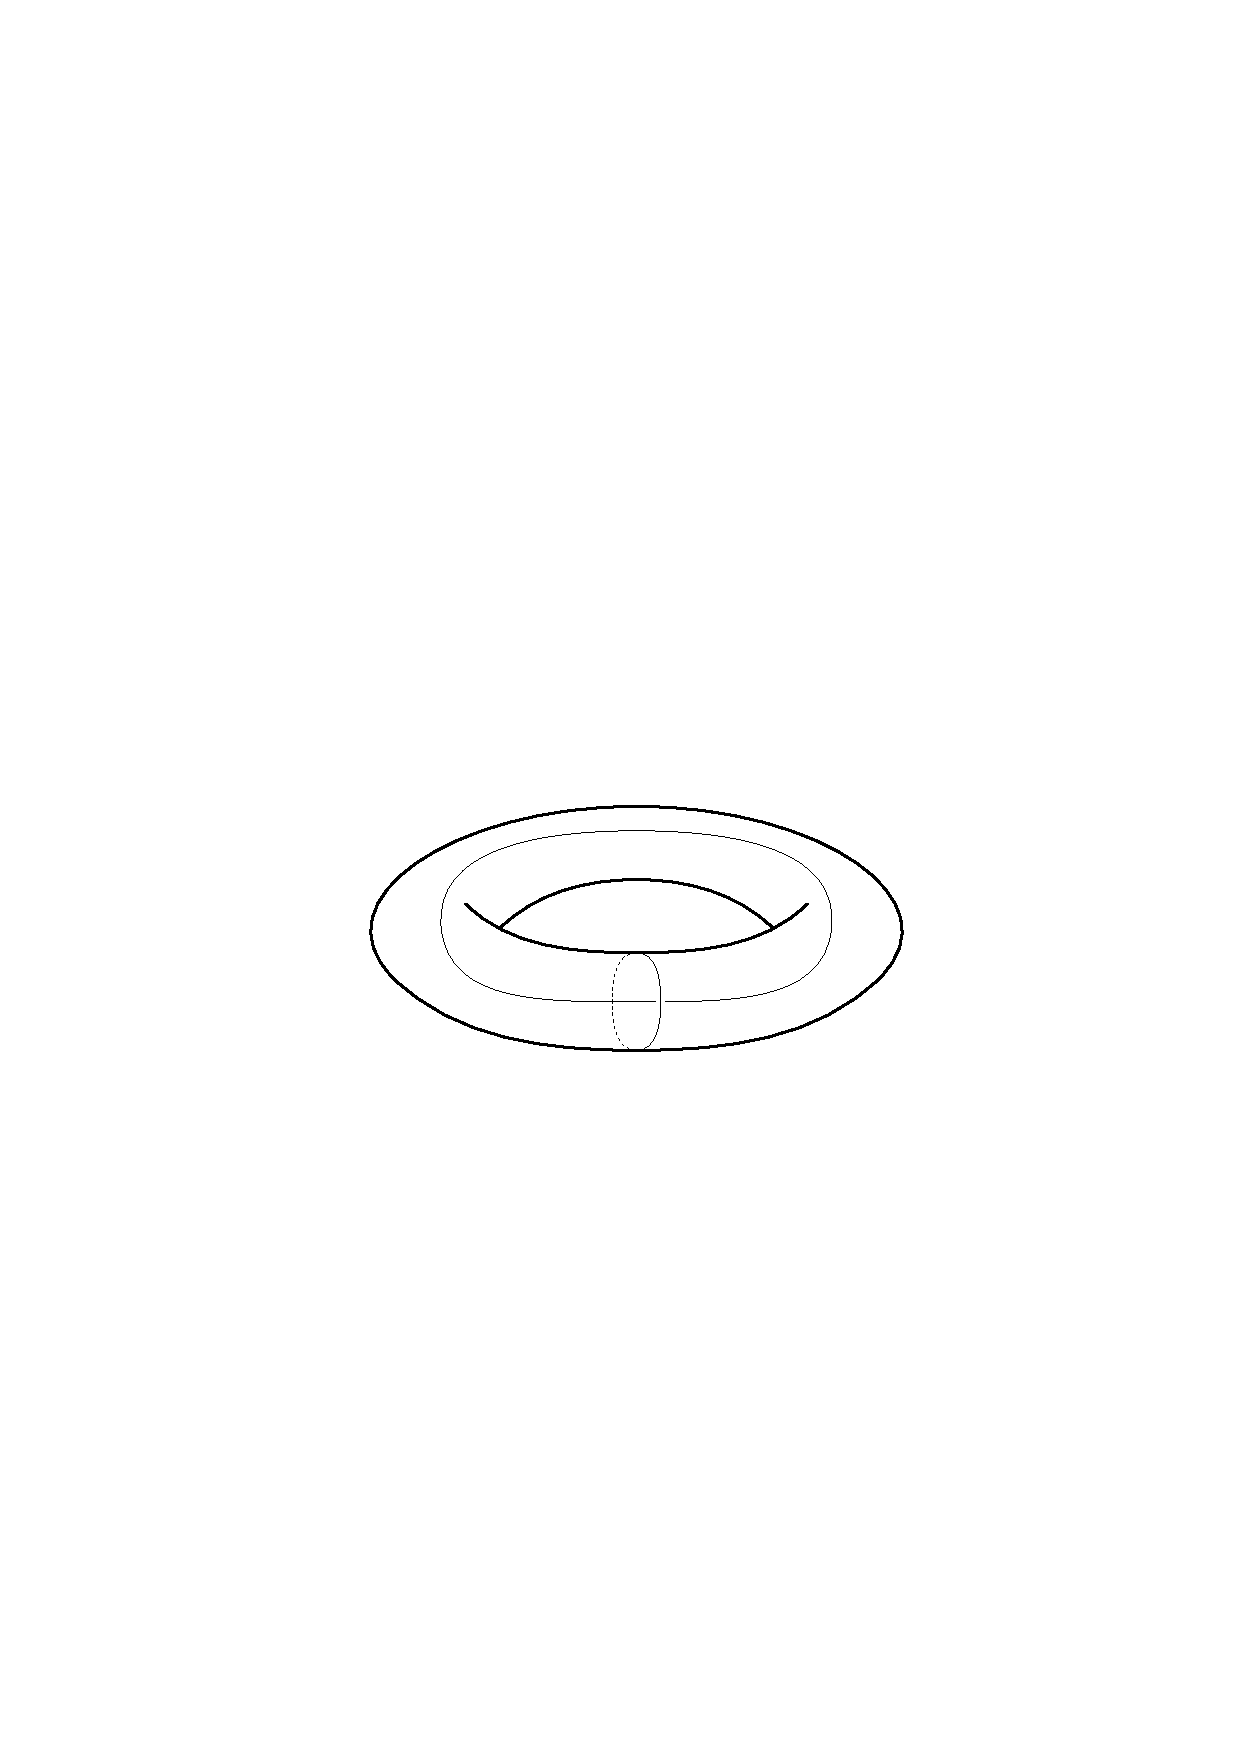
\includegraphics{chain_link_fence_knot_on_torus.pdf}
            \caption{Chain Link Fence Knot on a Torus}
            \label{fig:chain_link_fence_knot_on_torus}
        \end{figure}
        \par\hfill\par
        This last definition borrows the same difficulty from graph theory.
        While attaching handles at all of the $g$ virtual crossings yields an
        embedding into $M\times\mathbb{R}$ where $M$ is the compact orientable
        surface of genus $g$, it may have been possible to use fewer handles.
        Consider again Figs.~\ref{fig:graph_has_genus_001} and
        \ref{fig:graph_has_genus_002} where we created an embedding into the
        genus 3 compact surface. The starting graph was actually planar and
        needs no additional handles (Fig.~\ref{fig:graph_has_genus_003}).
        \begin{figure}
            \centering
            \resizebox{0.5\textwidth}{!}{%
                \includegraphics{graph_has_genus_003.pdf}
            }
            \caption{Planar Embedding}
            \label{fig:graph_has_genus_003}
        \end{figure}
        \par\hfill\par
        While it is possible to compute the minimal genus of a virtual knot,
        we will not need such an algorithm. Our later work will be motivated
        by a more classical problem which is related to this difficulty.
        If one is given an extended Gauss code (a \textit{virtual knot}),
        is it possible to determine if there is a (classical) knot diagram
        that realizes this code? We can indeed do this in linear time.
        \par\hfill\par
        A valid Gauss code with $2N$ entries describes a virtual knot with
        $N$ crossings. Suppose we have embedded our virtual knot into
        $M\times\mathbb{R}$ where $M$ is a compact orientable surface of
        minimal genus such that projecting down the $\mathbb{R}$ component
        yields a knot diagram on $M$ with the desired extended Gauss code.
        We thus obtain a graph embedded into $M$ where the crossings form the
        vertices. The graph is 4-valent so by the hand-shaking theorem there
        are $2N$ edges. We are in effect decomposing $M$ into a CW complex with
        $N$ 0-cells, $2N$ 1-cells, and $F$ 2-cells. If we can compute $F$ we
        will obtain $g$ via Euler's formula:
        \begin{equation}
            V-E+F=2-2g
        \end{equation}
        Substituting $V=N$ and $E=2N$ we have:
        \begin{equation}
            g=\frac{2+N-F}{2}
        \end{equation}
        Hence computing $F$ yields $g$, and if $g\ne{0}$ we will know the
        extended Gauss code does not describe the knot diagram of a
        classical knot. We now describe how to compute $F$.
        \par\hfill\par
        \begin{figure}
            \centering
            \includegraphics{thickened_crossings.pdf}
            \caption{Signed Thickened Crossings}
            \label{fig:thickened_crossings}
        \end{figure}
        Thicken the knot projection so that the crossings look like
        Fig.~\ref{fig:thickened_crossings}. Begin traveling along the thickened
        knot, following the orientation given by the Gauss code, and place your
        finger on the left wall at all times. When you come to a crossing,
        turn left so that your finger remains continuously on the wall of the
        thickened knot. Continue doing this until you return to your starting
        point. You will have just traced out a $k$-gon for some
        $k\in\mathbb{N}$. Attach a 2-cell by gluing along this polygon.
        Continue doing this until all $4N$ of the corners of the $N$ thickened
        crossings (again, appeal to Fig.~\ref{fig:thickened_crossings}) have
        been traveled. The total number of faces, which is the total number of
        cycles you've traveled, has now been computed. We require $4N$ steps,
        and so our algorithm does indeed run in linear time.
        \par\hfill\par
        The steps described translate to jumping between the entries in the
        Gauss code in a well-defined manner. \textit{Going left} means changing
        crossing type and then walking with or against the orientation.
        That is, if you come to entry \texttt{Ons}, with \texttt{n} the index
        and \texttt{s} the sign, jump ahead to \texttt{Uns}, changing crossing
        type. You then proceed to either the next entry in the Gauss code or
        the previous entry depending on the value of the sign \texttt{s}.
        This amounts to walking forwards or backwards. The correct direction
        can be computed from Fig.~\ref{fig:thickened_crossings}. If you are at
        the final entry and need to proceed forward, loop back around to the
        start. Similarly, if you are at the starting entry and need to move
        backwards, jump ahead to the end of the Gauss code. By repeatedly
        doing this we can compute the number of cycles and consequently
        calculate the genus.
        \par\hfill\par
        Applying this algorithm to the standard 3-crossing trefoil (either the
        left handed or right handed) will yield 5 faces, giving us a genus of
        0. The chain link fence knot \texttt{O0+ U1+ U0+ O1+} produces 2 faces,
        and so we end up with a genus 1 knot diagram which can be embedded on
        the torus. The faces, and the reason for the name
        \textit{chain link fence}, can be easily seen if we conduct our drawings
        on the flat torus (Fig.~\ref{fig:chain_link_fence_knot_on_flat_torus}).
        If we lift to the universal cover of the torus, which is the Euclidean
        plane, we can see the two aforementioned faces, as well as a chain
        link fence pattern
        (Fig.~\ref{fig:chain_link_fence_knot_on_flat_torus_universal_cover}).
        \begin{figure}
            \centering
            \includegraphics{chain_link_fence_knot_on_flat_torus.pdf}
            \caption{Chain Link Fence Virtual Knot on a Flat Torus}
            \label{fig:chain_link_fence_knot_on_flat_torus}
        \end{figure}
        \begin{figure}
            \centering
            \resizebox{\textwidth}{!}{%
                \includegraphics{%
                    chain_link_fence_knot_on_flat_torus_universal_cover.pdf
                }
            }
            \caption{Lift of the Chain Link Fence to the Universal Cover}
            \label{fig:chain_link_fence_knot_on_flat_torus_universal_cover}
        \end{figure}
        \par\hfill\par
        It should be considered a pleasant bonus if a knot invariant is also
        an invariant for virtual knots. It is especially enjoyable when an
        algorithm for a knot invariant can be copied for virtual knots with
        little or no additional effort. But, before proceeding, two warnings
        are worth mentioning.
        \par\hfill\par
        The operations of the Reidemeister moves are stricter for virtual knots
        via extended Gauss code. For classical knots, should we find
        \texttt{On Om} followed by \texttt{Un Um}, or any re-ordering thereof,
        we can apply Type II and delete the four entries from the code. This is
        not so for virtual knots. Indeed, were it true the chain link fence
        would be equivalent to the unknot. The sign is crucial for a correct
        description of Type II moves in the virtual setting. For a true
        Type II move, the signs alternate. This in agreement with the fact that
        Type II does not change the writhe of a diagram. So, should we find
        \texttt{On+ Om-} followed by \texttt{Un+ Um-}, or any re-ordering
        thereof, we may apply Type II and delete the four entries, be it a
        classical or virtual knot.
        \par\hfill\par
        Lastly, the algorithm described previously computed the genus of a
        virtual knot \textit{diagram}, and not the minimal genus of all
        possible equivalent diagram. By application of Type II it is possible
        give the right-handed trefoil a genus 1 knot diagram, for example
        \texttt{O0+ U1+ O2+ O3- O4+ U0+ U3- U2+ O1+ U4+}. The Reidemeister
        moves may change the genus of a diagram.
    \subsection{Planar Diagrams}
        Planar diagram code, commonly called PD code, is one of the more popular
        representations found in programming libraries. We start with an
        oriented knot diagram and pick a starting point. We follow the
        orientation and label the \textit{arcs}, the edges between crossings,
        in increasing order from $0$ to $2N-1$ where $N$ is the number of
        crossings. Once the arcs have been labeled we once again walk around
        the knot diagram and each time we come to an under crossing we write
        down \texttt{X[a,b,c,d]} where \texttt{a} is the number of the arc you
        are coming from, \texttt{c} is the arc you'll be leaving through,
        \texttt{b} is the arc to your \textit{right}, and \texttt{d} is the
        arc to your \textit{left}. The PD code of the diagram is the ordered
        sequence of 4-tuples \texttt{X[a,b,c,d]} for each under crossing you
        encounter in the order you encounter them. Using
        Fig.~\ref{fig:trefoil_knot_arcs_labeled}, the right-handed trefoil can
        represented by writing \texttt{X[1,5,2,4],X[3,1,4,0],X[5,3,0,2]}.
        \begin{figure}
            \centering
            \includegraphics{trefoil_knot_arcs_labeled.pdf}
            \caption{Trefoil Knot with Arcs Labeled}
            \label{fig:trefoil_knot_arcs_labeled}
        \end{figure}
        \par\hfill\par
        Planar diagram code can recover unsigned Gauss code, but moreover
        the sign of the crossings can also be computed. Since the arcs are in
        increasing order, we have that for each entry
        \texttt{X[a,b,c,d]}, the difference $\texttt{c}-\texttt{a}$ is either
        1 or $1-N$, with $1-N$ occurring if and only of \texttt{a} is the final
        arc in the ordering. In contrast, the difference $\texttt{b}-\texttt{d}$
        can be $+1$ or $-1$, once reduced mod $N$. $+1$ means the crossing is
        positive and $-1$ means the crossing is negative. We can see this by
        appealing to the rigorous definition of the sign. The over strand can
        be chosen to represent the positive $x$ axis. If
        $\texttt{b}-\texttt{d}=+1$ this means the under strand is pointing
        into the upper half plane, and so the determinant will be
        positive. Similarly $\texttt{b}-\texttt{d}=-1$ means the under strand
        points into the lower half plane, the opposite orientation, and so
        the determinant is negative. Whether this is a
        lucky coincidence, or if the signing of the crossings was originally
        chosen to yield this result, one must admit it is a rather elegant
        computation.
        \par\hfill\par
        Since the signs of the crossings can be computed, and since
        PD code can determine the unsigned Gauss code, we immediately see that
        PD code and extended Gauss code have the same information. Because of
        this one may use PD codes for virtual knots as well, but the phrasing
        \textit{virtual planar diagram code} is rather unfortunate for
        non-planar virtual knot diagrams. At any rate, it is \textit{not}
        common practice to use PD codes to represent virtual knots. Indeed,
        some programming libraries have checks to ensure the input PD code
        represents a planar knot diagram before allowing computations to be
        performed.
    \subsection{Dowker-Thistlethwaite Notation}
        Dowker-Thistlethwaite code (DT code for short) compactly describes
        knots. Because of this it is used in tabulation efforts where millions
        of distinct knot are listed in massive tables
        (see, for example \cite{Burton2020TheN3} and \cite{regina}).
        \par\hfill\par
        Start with an oriented knot diagram and choose a starting point.
        Walk along the knot, following the orientation, and number the
        crossings as you pass them in increasing order. For each odd number,
        if you are on the under strand as you pass the crossing,
        prepend a minus sign. Should you come upon a crossing you've already
        marked, label it again with the second number as well.
        At the end you should have a permutation of all numbers (with possible
        minus signs) between $0$ and $2N-1$ where $N$ is the number of
        crossings, each crossing having two numbers assigned to it. If the knot
        diagram is \textit{planar} and represents a classical knot, by a
        parity argument and the Jordan curve theorem we see that each crossing
        will have one odd number and one even number associated to it. Pair
        the numbers together into tuples $(2n,\,\pm(2m+1))$ corresponding to the
        same crossing. Lastly, order the tuples lexicographically by giving
        preference to the first entry (the even number in the tuple).
        The DT code is the corresponding ordered sequence of odd numbers,
        with minus signs included.\footnote{%
            In computer science it is very common to start numbering at zero,
            which is what we have done several times throughout. In the
            original paper the labeling starts at 1. Because of this the
            \textit{even} numbers are given plus and minus signs, and the
            tuples are ordered with respect to the \textit{odd} numbers. A
            minor change, but a very important one. Failure to be consistent
            can result in the wrong DT code.
        }
        \par\hfill\par
        Quite verbose, let us consider an example.
        Fig.~\ref{fig:trefoil_knot_oriented_001} depicts an oriented
        right-handed trefoil, let's start with this. Choosing the top-most
        point, we obtain the sequence of ordered tuples
        $(0,\,3)$, $(2,\,5)$, $(4,\,1)$. So our DT code for the right-handed
        trefoil is \texttt{3 5 1}. The same DT code is attainable for the
        left-handed trefoil, meaning the notation is mirror insensitive. Still,
        it is extremely compact. The following theorem further justifies its
        use.
        \begin{theorem}[Dowker, Thistlethwaite 1983]
            If two prime knots have the same DT code, then they are either
            equivalent or are mirrors of one another.
        \end{theorem}
        \begin{proof}
            See \cite{DOWKER198319}.
        \end{proof}
        Since knot tabulation rarely differentiates between mirrors, and
        almost exclusively concerns itself with the listing of prime knots,
        DT code is perfect for such an endeavor.
        \par\hfill\par
        Since the code consists entirely of odd numbers we can obtain the
        \textbf{simplified DT code} by subtracting one and dividing by two,
        doing this to each element. The trefoil then becomes
        \texttt{1 2 0}. Furthermore, should we be concerned with knots of
        no more than 26 crossings, we can substitute numbers with letters.
        This is the \textbf{alphabetical DT code}. The trefoil becomes
        \texttt{bca}. Should a minus sign be part of the original DT code
        we would add one and divide by two for the simplified code, and the
        alphabetical code would be given using a capital letter. For example,
        the knot $8_{19}$ in the Rolfsen table
        has the alphabetical DT code \texttt{bdFaGHCE}. In our presentation of
        knot tables for \textit{classical knots} we will exclusively use the
        alphabetical DT notation for its brevity. For virtual knots DT code is
        undefined. It is not the case that each crossing must have an even and
        odd number associated to it. Consider the chain link fence knot
        \texttt{O0+ U1+ U0+ O1+}, the tuples are $(0,\,2)$ for the zeroth
        crossing and $(1,\,3)$ for the first one. We must abandon DT code when
        in the virtual setting.
        \par\hfill\par
    \subsection{Braids}
        Braids are one of the original mathematical means of representing knots,
        the term braid being coined by Emil Artin in 1925
        \cite{ArtinBraidTheory1925}, with the theory being powered by
        Alexander's theorem which we'll now discuss. We start with $2N$
        points, $N$ on the line $x=0$ and $N$ on the line $x=1$, with points
        pairing off in equal heights. Given a point on the $x=0$ line we are
        presented with two options:
        \begin{enumerate}
            \item Draw a straight line across to the point on the line $x=1$
                with the same height.
            \item Draw a line to the point directly below this, or directly
            above this. If a crossing occurs with an already drawn line,
            indicate which is over and which is under.
        \end{enumerate}
        \begin{figure}
            \centering
            \includegraphics{braid_two_strand_example_001.pdf}
            \caption{Braid with Two Strands}
            \label{fig:braid_two_strand_example_001}
        \end{figure}
        We can then place $N$ more points on the line $x=2$ with the same
        heights and repeat this process. Concatenating the elementary moves
        can yield very complicated objects as we iterate this process more.
        The underlying structure is that of a finitely presented group with
        one generator for each starting point. The element
        $\sigma_{k}$ represents the line going from
        $k$ to $k+1$, passing \textit{over} the passing from $k+1$ to $k$.
        The inverse reverses this order. We then consider these \textit{braids}
        up to equivalence via Reidemeister moves. This yields the following
        presentation.
        \begin{definition}[\textbf{Braid Group}]
            The braid group on $N\in\mathbb{N}^{+}$ strands is group $B_{N}$
            with presentation:
            \begin{equation}
                B_{N}=\{\,
                    \sigma_{0},\,\dots,\,\sigma_{N-2}\;|\;
                    \sigma_{j}\sigma_{j+1}\sigma_{j}
                    =\sigma_{j+1}\sigma_{j}\sigma_{j+1},\,
                    \sigma_{k}\sigma_{\ell}=\sigma_{\ell}\sigma_{k}\,
                \}
            \end{equation}
            for all $0\leq{j}\leq{N-3}$ and all $k,\,\ell$ satisfying
            $|k-\ell|\geq{2}$.
        \end{definition}
        \begin{figure}
            \centering
            \includegraphics{braid_closure_hopf_link_001.pdf}
            \caption{Braid Closure for the Hopf Link}
            \label{fig:braid_closure_hopf_link_001}
        \end{figure}
        The first three examples of braid groups are well studied:
        $B_{1}$ is trivial, $B_{2}$ is isomorphic to $\mathbb{Z}$, and
        $B_{}$ is isomorphic to the fundamental group of the complement of
        the trefoil knot in $\mathbb{R}^{3}$. By \textit{closing} up the
        braid, connecting the dot on the left most line with the dot on the
        right most line of the same height via a circular arc that goes up and
        around, we obtain a link, the \textbf{braid closure} of the braid.
        Closing up the previous example yields the Hopf link
        (Fig.~\ref{fig:braid_closure_hopf_link_001}).
        All knots an links arise in such a way.
        \begin{theorem}[\textbf{Alexander's Theorem}]
            If $\mathcal{K}$ is a knot (or link) type, then there is a
            positive integer $N\in\mathbb{N}^{+}$ and an element
            $g\in{B}_{N}$ such that the braid closure of $g$ yields a
            knot diagram for $\mathcal{K}$.
        \end{theorem}
        \begin{proof}
            See \cite{AlexandersTheorem1923}.
        \end{proof}
        Braids will mostly play a small part in this work, but
        several programming libraries have tools dedicated to their
        investigations.
    \subsection{Tait Graphs}
        The last representation we wish to describe is one of the original
        ones: the \textbf{Tait graph}.

        \section{Knot Polynomials}
            \subsection{Alexander Polynomial}
            \subsection{Kauffman Bracket}
            \subsection{Jones Polynomial}
        \section{Khovanov Homology}
        \section{Knot Recognition}
    \chapter{Contact Topology}
        \section{Contact Structures}
        \section{Legendrian Knot Invariants}
        \section{Legendrian Simple Knots}
    \chapter{Algorithms and Computation}
        \section{Algorithms for the Jones Polynomial}
        \section{Computation of Khovanov Homology}
        \section{The HOMFLY-PT Polynomial}
    \chapter{Numerical Results}
        \section{Torus Knots}
        \section{Twist Knots}
        \section{Conjectured Legendrian Simple Knots}
        \section{Relative Strengths of Knot Invariants}
    \clearpage
    \nocite{*}
    \bibliographystyle{annotate}
    \bibliography{bib.bib}
\end{document}
